\documentclass[mathserif]{beamer}

\usepackage[english]{babel} % language selection: english/ngerman
                            % note: delete all output files on language change
\usepackage[utf8]{inputenc} % allow for using umlauts
\usepackage{lipsum}         % provide lorem ipsum ...
\usepackage{siunitx}        % provide SI units
\usepackage{amsfonts}       % Provides hollow R for real numbers, hollow C for complex numbers, etc.
\usepackage{algorithm}      % Provides Border for Pseudocode
\usepackage{algpseudocode}  % Provides Pseudocode
\usepackage{interval}       % Provides proper intervals
\usepackage{listings}       % Provides Source Code Listing
\usepackage{gensymb}        % Provides the degree symbol
\usepackage{wrapfig}        % Provides wrapping of text around figures
\usepackage{amssymb}        % Provides empty set symbol (\varnothing)
\usepackage{colortbl}
\usepackage{varwidth}
\usepackage{xcolor}
\usepackage{mathtools}
\usepackage[export]{adjustbox}
\usepackage{subfig}
\usepackage{tikz}
\usepackage{slashbox}
\usepackage{hyperref}
\usepackage{esvect}
\usepackage[makeroom]{cancel}
\usepackage{pdfpages}
\usepackage{amsmath}
\usepackage{outlines}
\usepackage{kbordermatrix}
\usepackage[customcolors]{hf-tikz}

\usetikzlibrary{arrows.meta}

\tikzset{
    style green/.style={
    set fill color=green!60!lime!40,
    set border color=white,
  },
  style cyan/.style={
    set fill color=cyan!90!blue!60,
    set border color=white,
  },
  style red/.style={
    set fill color=red!30,
    set border color=white,
  },
  style orange/.style={
    set fill color=orange!80!red!40,
    set border color=white,
  },
  hor/.style={
    above left offset={-0.15,0.31},
    below right offset={0.15,-0.10},
    #1
  },
  ver/.style={
    above left offset={-0.10,0.35},
    below right offset={0.10,-0.15},
    #1
  }
}

%\usepackage[T1]{fontenc}
%\usepackage[tt=false,osf]{libertinus}
%\usepackage{inconsolata}

\usetheme[progressbar=frametitle]{metropolis}
%\setbeamertemplate{frame numbering}[fraction]
%\useoutertheme{metropolis}
%\useinnertheme{metropolis}
%\usefonttheme{metropolis}
%\usecolortheme{spruce}
%\setbeamercolor{background canvas}{bg=white}
\metroset{block=fill}

\title{Gerichtete Graphen}
%\subtitle{Gerichtete Graphen}

\author{Nico Pistel}
% - Give the names in the same order as the appear in the paper.
% - Use the \inst{?} command only if the authors have different
%     affiliation.

\institute[Institute] % (optional, but mostly needed)
{
    Fachbereich Wirtschaft und Informationstechnik\\
    Westfälische Hochschule Bocholt
}

\date{Diskrete Mathematik und Stochastik, 2019}
% - Either use conference name or its abbreviation.
% - Not really informative to the audience, more for people (including
%     yourself) who are reading the slides online

\subject{Subject}
% This is only inserted into the PDF information catalog. Can be left
% out.

% If you have a file called "university-logo-filename.xxx", where xxx
% is a graphic format that can be processed by latex or pdflatex,
% resp., then you can add a logo as follows:

\pgfdeclareimage[height=0.5cm]{university-logo}{img/wh.png}
\logo{\pgfuseimage{university-logo}}

% Delete this, if you do not want the table of contents to pop up at
% the beginning of each subsection:
%\AtBeginSubsection[]
%{
%    \begin{frame}<beamer>{Outline}
%        \tableofcontents[currentsection,currentsubsection]
%    \end{frame}
%}

% Let's get started
\begin{document}

\begin{frame}
    \titlepage
\end{frame}

\begin{frame}{Outline}
    \tableofcontents
    % You might wish to add the option [pausesections]
\end{frame}

% Section and subsections will appear in the presentation overview
% and table of contents.
\section{First Main Section}

\subsection{First Subsection}

\begin{frame}{First Slide Title}{Optional Subtitle}
    \begin{itemize}
    \item {
        My first point.
    }
    \item {
        My second point.
    }
    \end{itemize}
\end{frame}

\subsection{Second Subsection}

% You can reveal the parts of a slide one at a time
% with the \pause command:
\begin{frame}{Second Slide Title}
    \begin{itemize}
    \item {
        First item.
        \pause % The slide will pause after showing the first item
    }
    \item {
        Second item.
    }
    % You can also specify when the content should appear
    % by using <n->:
    \item<3-> {
        Third item.
    }
    \item<4-> {
        Fourth item.
    }
    % or you can use the \uncover command to reveal general
    % content (not just \items):
    \item<5-> {
        Fifth item. \uncover<6->{Extra text in the fifth item.}
    }
    \end{itemize}
\end{frame}

\section{Topologisches Sortieren}
\subsection{Beispiel: Topologisches Sortieren}
\begin{frame}{Beispiel: Topologisches Sortieren}
    \centering
    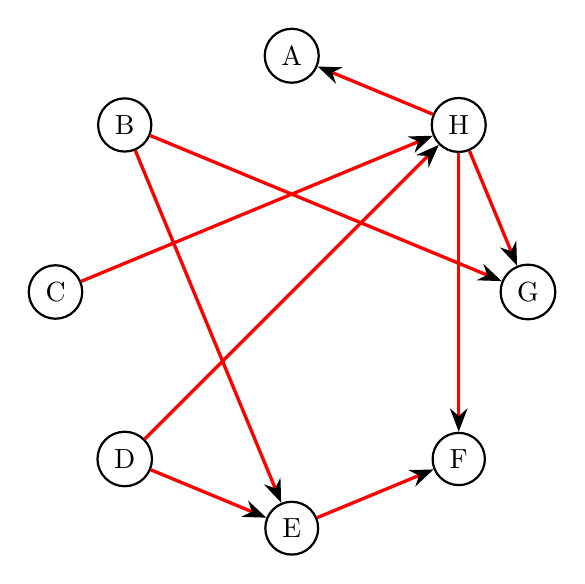
\begin{tikzpicture}
        \begin{scope}[every node/.style={circle,thick,draw}]
            \node (A) at (0 + 3 *  0    , 0 + 3 *  1    ) {A};
            \node (B) at (0 + 3 * -0.707, 0 + 3 *  0.707) {B};
            \node (C) at (0 + 3 * -1    , 0 + 3 *  0    ) {C};
            \node (D) at (0 + 3 * -0.707, 0 + 3 * -0.707) {D};
            \node (E) at (0 + 3 *  0    , 0 + 3 * -1    ) {E};
            \node (F) at (0 + 3 *  0.707, 0 + 3 * -0.707) {F};
            \node (G) at (0 + 3 *  1    , 0 + 3 *  0    ) {G};
            \node (H) at (0 + 3 *  0.707, 0 + 3 *  0.707) {H};
        \end{scope}
        \begin{scope}[>={Stealth[black]}, every edge/.style={draw=red,very thick}]
            \path [->] (B) edge (E);
            \path [->] (B) edge (G);

            \path [->] (C) edge (H);

            \path [->] (D) edge (E);
            \path [->] (D) edge (H);

            \path [->] (E) edge (F);

            \path [->] (H) edge (A);
            \path [->] (H) edge (F);
            \path [->] (H) edge (G);
        \end{scope}
    \end{tikzpicture}
\end{frame}
\begin{frame}{Beispiel: Topologisches Sortieren}
    \centering
    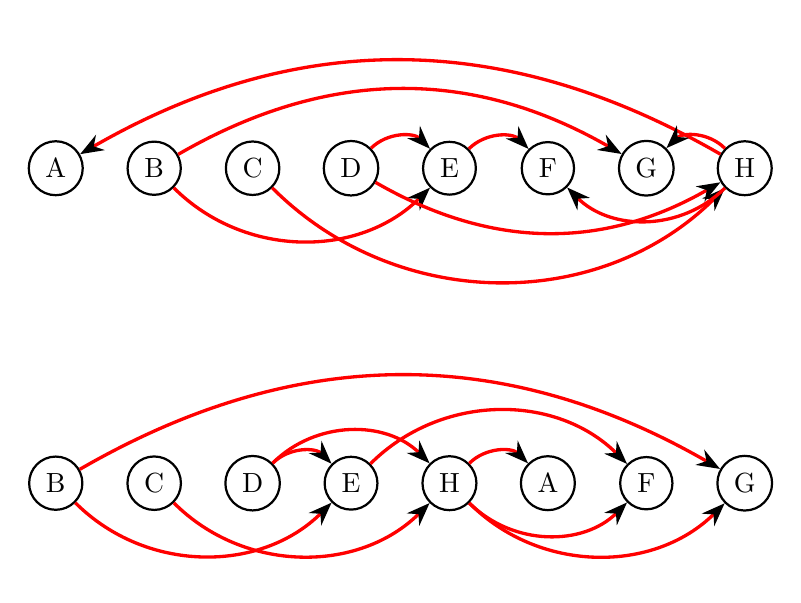
\begin{tikzpicture}
        \begin{scope}[every node/.style={circle,thick,draw}]
            \node (B) at (0.00, -1) {B};
            \node (C) at (1.25, -1) {C};
            \node (D) at (2.50, -1) {D};
            \node (E) at (3.75, -1) {E};
            \node (H) at (5.00, -1) {H};
            \node (A) at (6.25, -1) {A};
            \node (F) at (7.50, -1) {F};
            \node (G) at (8.75, -1) {G};

            \node (Ap) at (0.00, 3) {A};
            \node (Bp) at (1.25, 3) {B};
            \node (Cp) at (2.50, 3) {C};
            \node (Dp) at (3.75, 3) {D};
            \node (Ep) at (5.00, 3) {E};
            \node (Fp) at (6.25, 3) {F};
            \node (Gp) at (7.50, 3) {G};
            \node (Hp) at (8.75, 3) {H};
        \end{scope}
        \begin{scope}[>={Stealth[black]}, every edge/.style={draw=red,very thick}]
            \path [->] (B) edge[bend right=45] (E);
            \path [->] (B) edge[bend right=-30] (G);

            \path [->] (C) edge[bend right=45] (H);

            \path [->] (D) edge[bend right=-45] (E);
            \path [->] (D) edge[bend right=-45] (H);

            \path [->] (E) edge[bend right=-45] (F);

            \path [->] (H) edge[bend right=-45] (A);
            \path [->] (H) edge[bend right=45] (F);
            \path [->] (H) edge[bend right=45] (G);


            \path [->] (Bp) edge[bend right=45] (Ep);
            \path [->] (Bp) edge[bend right=-30] (Gp);

            \path [->] (Cp) edge[bend right=45] (Hp);

            \path [->] (Dp) edge[bend right=-45] (Ep);
            \path [->] (Dp) edge[bend right=30] (Hp);

            \path [->] (Ep) edge[bend right=-45] (Fp);

            \path [->] (Hp) edge[bend right=30] (Ap);
            \path [->] (Hp) edge[bend right=-45] (Fp);
            \path [->] (Hp) edge[bend right=45] (Gp);
        \end{scope}
    \end{tikzpicture}
\end{frame}
\subsection{Kahn's Algorithmus}
\begin{frame}{Kahn's Algorithmus}
    jo
\end{frame}
\begin{frame}{Beispiel: Kahn's Algorithmus}
    \begin{columns}
        \begin{column}{0.70\textwidth}
            \alt<10->{
                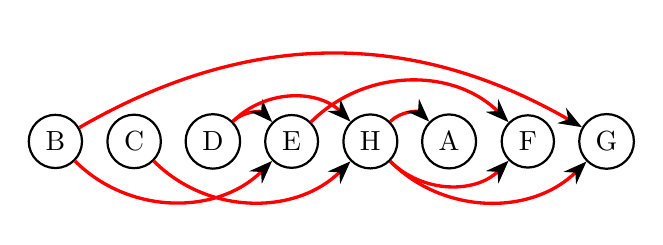
\begin{tikzpicture}
                    \begin{scope}[every node/.style={circle,thick,draw}]
                        \onslide<11->{\node (B) at (0.00, 0) {B};}
                        \onslide<14->{\node (C) at (1.00, 0) {C};}
                        \onslide<17->{\node (D) at (2.00, 0) {D};}
                        \onslide<20->{\node (E) at (3.00, 0) {E};}
                        \onslide<23->{\node (H) at (4.00, 0) {H};}
                        \onslide<26->{\node (A) at (5.00, 0) {A};}
                        \onslide<28->{\node (F) at (6.00, 0) {F};}
                        \onslide<30->{\node (G) at (7.00, 0) {G};}
                    \end{scope}
                    \begin{scope}[>={Stealth[black]}, every edge/.style={draw=red,very thick}]
                        \onslide<20->{\path [->] (B) edge[bend right=45] (E);}
                        \onslide<30->{\path [->] (B) edge[bend right=-30] (G);}

                        \onslide<23->{\path [->] (C) edge[bend right=45] (H);}

                        \onslide<20->{\path [->] (D) edge[bend right=-45] (E);}
                        \onslide<23->{\path [->] (D) edge[bend right=-45] (H);}

                        \onslide<28->{\path [->] (E) edge[bend right=-45] (F);}

                        \onslide<26->{\path [->] (H) edge[bend right=-45] (A);}
                        \onslide<28->{\path [->] (H) edge[bend right=45] (F);}
                        \onslide<30->{\path [->] (H) edge[bend right=45] (G);}
                    \end{scope}
                \end{tikzpicture}
            }{
                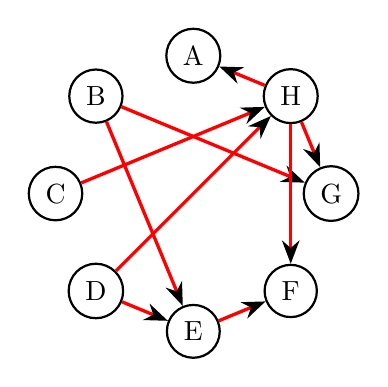
\begin{tikzpicture}
                    \begin{scope}[every node/.style={circle,thick,draw}]
                        \node (A) at (0 + 1.75 *  0    , 0 + 1.75 *  1    ) {A};
                        \node (B) at (0 + 1.75 * -0.707, 0 + 1.75 *  0.707) {B};
                        \node (C) at (0 + 1.75 * -1    , 0 + 1.75 *  0    ) {C};
                        \node (D) at (0 + 1.75 * -0.707, 0 + 1.75 * -0.707) {D};
                        \node (E) at (0 + 1.75 *  0    , 0 + 1.75 * -1    ) {E};
                        \node (F) at (0 + 1.75 *  0.707, 0 + 1.75 * -0.707) {F};
                        \node (G) at (0 + 1.75 *  1    , 0 + 1.75 *  0    ) {G};
                        \node (H) at (0 + 1.75 *  0.707, 0 + 1.75 *  0.707) {H};
                    \end{scope}
                    \begin{scope}[>={Stealth[black]}, every edge/.style={draw=red,very thick}]
                        \path [->] (B) edge (E);
                        \path [->] (B) edge (G);

                        \path [->] (C) edge (H);

                        \path [->] (D) edge (E);
                        \path [->] (D) edge (H);

                        \path [->] (E) edge (F);

                        \path [->] (H) edge (A);
                        \path [->] (H) edge (F);
                        \path [->] (H) edge (G);
                    \end{scope}
                \end{tikzpicture}
            }
        \end{column}
        \begin{column}{0.30\textwidth}
            \begin{tabular}{c|c|c}
                $i$ & $v$ & $A(v)$ \\
                \hline
                \onslide<25>{\tikzmarkin[ver=style green]{r6}}\onslide<26->{$6$} & A & \onslide<2->{$\{\alt<24->{\cancel{\text{H}}}{\text{H}}\}$}\onslide<25>{\tikzmarkend{r6}} \\
                \onslide<10-11>{\tikzmarkin[ver=style green]{r1}}\onslide<11->{$1$} & B & \onslide<3->{$\varnothing$}\onslide<10-11>{\tikzmarkend{r1}} \\
                \onslide<13-14>{\tikzmarkin[ver=style green]{r2}}\onslide<14->{$2$} & C & \onslide<4->{$\varnothing$}\onslide<13-14>{\tikzmarkend{r2}} \\
                \onslide<16-17>{\tikzmarkin[ver=style green]{r3}}\onslide<17->{$3$} & D & \onslide<5->{$\varnothing$}\onslide<16-17>{\tikzmarkend{r3}} \\
                \onslide<19-20>{\tikzmarkin[ver=style green]{r4}}\onslide<20->{$4$} & E & \onslide<6->{$\{\alt<12->{\cancel{\text{B}}}{\text{B}},\alt<18->{\cancel{\text{D}}}{\text{D}}\}$}\onslide<19-20>{\tikzmarkend{r4}} \\
                \onslide<27>{\tikzmarkin[ver=style green]{r7}}\onslide<28->{$7$} & F & \onslide<7->{$\{\alt<21->{\cancel{\text{E}}}{\text{E}},\alt<24->{\cancel{\text{H}}}{\text{H}}\}$}\onslide<27>{\tikzmarkend{r7}} \\
                \onslide<29>{\tikzmarkin[ver=style green]{r8}}\onslide<30->{$8$} & G & \onslide<8->{$\{\alt<12->{\cancel{\text{B}}}{\text{B}},\alt<24->{\cancel{\text{H}}}{\text{H}}\}$}\onslide<29>{\tikzmarkend{r8}} \\
                \onslide<22-23>{\tikzmarkin[ver=style green]{r5}}\onslide<23->{$5$} & H & \onslide<9->{$\{\alt<15->{\cancel{\text{C}}}{\text{C}},\alt<18->{\cancel{\text{D}}}{\text{D}}\}$}\onslide<22-23>{\tikzmarkend{r5}} \\
            \end{tabular}
        \end{column}
    \end{columns}
\end{frame}
\section{Wege in Digraphen}
\begin{frame}{Wege in Digraphen}
    \begin{itemize}
        \item Existenz von Wegen zwischen beliebigen Knoten
        \item Adjazenzmatrix $\mathbf{M}\longrightarrow$ Erreichbarkeitsmatrix $\mathbf{M}^*$
        \item Kantenrelation $E\longrightarrow$ transitiver Abschluss $E^*$
    \end{itemize}
\end{frame}
\subsection{Wege als transitiver Abschluss der Kantenrelation}
\begin{frame}{Wege als transitiver Abschluss der Kantenrelation}
    \begin{itemize}
        \item Kantenrelation $E$: Menge von Wegen der Länge $1$ zwischen Knoten
        \item Menge von Wegen der Länge $2$ als Komposition von $E$ mit sich selber:\\$E\circ E=\{(v_1,v_2)\in V^2|\exists u\in V:(v_1,u)\in E\land(u,v_2)\in E\}$
        \item Menge von Wegen einer Länge $k$: $\underbrace{E\circ\dots\circ E}_{k\text{ mal}}$
        \item Transitiver Abschluss als Vereinigung dieser Mengen:\\$E^*=E\cup E\circ E\cup\dots\cup\underbrace{E\circ\dots\circ E}_{n\text{ mal}}$
    \end{itemize}
\end{frame}
\begin{frame}{Potenzieren der Adjazenzmatrix}
    \begin{outline}
        \1 Komposition von $E$ als logisches Matrixprodukt der Adjazenzmatrix $\mathbf{M}$
        \1 Weitere Komposition durch das Potenzieren von $\mathbf{M}$
        \1 Vereinigen der Mengen durch das logische \textbf{oder} der Matrizen
        \1 Logisches \textbf{oder} zweier Matrizen wird komponentenweise gebildet
        \2 $(\mathbf{A}\lor\mathbf{B})_{ij}=\mathbf{A}_{ij}\lor\mathbf{B}_{ij}$
    \end{outline}
    \begin{block}{Berechnung der Erreichbarkeitsmatrix $\mathbf{M}^*$}
        \[\mathbf{M}^*=\mathbf{M}\lor\mathbf{M}^2\lor\dots\lor\mathbf{M}^n\]
    \end{block}
\end{frame}
\begin{frame}{Beispiel: Potenzieren der Adjazenzmatrix}
    \begin{columns}
        \begin{column}[t]{0.25\textwidth}
            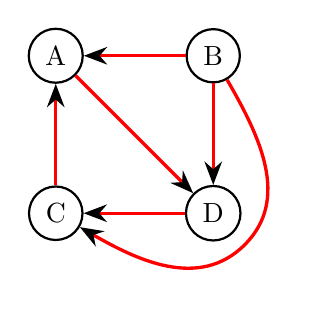
\begin{tikzpicture}
                \begin{scope}[every node/.style={circle,thick,draw}]
                    \node (A) at (0,2) {A};
                    \node (B) at (2,2) {B};
                    \node (C) at (0,0) {C};
                    \node (D) at (2,0) {D};
                \end{scope}
                \begin{scope}[>={Stealth[black]}, every edge/.style={draw=red,very thick}]
                    \path [->] (A) edge (D);
                    \path [->] (B) edge (A);
                    \path [->] (B) edge (D);
                    \path [->] (C) edge (A);
                    \path [->] (D) edge (C);
                    \draw [very thick,draw=red,->] (B) to[out=-60,in=45] (2.40,-0.40) to[out=-135,in=-30] (C);
                \end{scope}
            \end{tikzpicture}
        \end{column}
        \begin{column}{0.70\textwidth}
            \small
            \begin{align*}
                \mathbf{M}&=\kbordermatrix{
                               & \text{A} & \text{B} & \text{C} & \text{D} \\
                      \text{A} &        0 &        0 &        0 &        1 \\
                      \text{B} &        1 &        0 &        1 &        1 \\
                      \text{C} &        1 &        0 &        0 &        0 \\
                      \text{D} &        0 &        0 &        1 &        0
                }
                &\mathbf{M}^2&=\kbordermatrix{
                               & \text{A} & \text{B} & \text{C} & \text{D} \\
                      \text{A} &        0 &        0 &        1 &        0 \\
                      \text{B} &        1 &        0 &        1 &        1 \\
                      \text{C} &        0 &        0 &        0 &        1 \\
                      \text{D} &        1 &        0 &        0 &        0
                }\\
                \mathbf{M}^3&=\kbordermatrix{
                               & \text{A} & \text{B} & \text{C} & \text{D} \\
                      \text{A} &        1 &        0 &        0 &        0 \\
                      \text{B} &        1 &        0 &        1 &        1 \\
                      \text{C} &        0 &        0 &        1 &        0 \\
                      \text{D} &        0 &        0 &        0 &        1
                }
                &\mathbf{M}^4&=\kbordermatrix{
                               & \text{A} & \text{B} & \text{C} & \text{D} \\
                      \text{A} &        0 &        0 &        0 &        1 \\
                      \text{B} &        1 &        0 &        1 &        1 \\
                      \text{C} &        1 &        0 &        0 &        0 \\
                      \text{D} &        0 &        0 &        1 &        0
                }
            \end{align*}
            \[\mathbf{M}^*=\kbordermatrix{
                         & \text{A} & \text{B} & \text{C} & \text{D} \\
                \text{A} &        1 &        0 &        1 &        1 \\
                \text{B} &        1 &        0 &        1 &        1 \\
                \text{C} &        1 &        0 &        1 &        1 \\
                \text{D} &        1 &        0 &        1 &        1
            }\]
        \end{column}
    \end{columns}
\end{frame}
\subsection{Warshall's Algorithmus}
\begin{frame}{Warshall's Algorithmus}
    \begin{outline}
        \1 Matrixmultiplikation ist aufwändig
        \2 Berechnen der Potenzen bei Graphen mit vielen Knoten ist problematisch
        \1 Warshall ermittelt $\mathbf{M}^*$ in Worst-Case $\Theta(n^3)$ Zeit
        \1 Warshall's Algorithmus arbeitet \textit{In-Place}
        \2 $\mathbf{M}$ wird iterativ in $\mathbf{M}^*$ überführt
        \1 Warshall erzeugt Matrizen $\mathbf{W}_0,\mathbf{W}_1,\dots,\mathbf{W}_n$
        \2 Wobei $\mathbf{W}_0=\mathbf{M}$ und $\mathbf{W}_n=\mathbf{M}^*$
        \1 $\mathbf{W}_k[i,j]=1\Longleftrightarrow$ Es existiert ein Weg von $v_i$ nach $v_j$, wobei alle Zwischenknoten $\in\{v_1,v_2,\dots,v_k\}$ sind
    \end{outline}
\end{frame}
\begin{frame}{Pseudocode: Warshall's Algorithmus}
    \begin{algorithm}[H]
        \caption{Warshall's Algorithmus}
        \begin{algorithmic}[1]
            \Function{Warshall}{$M$}
                \State $W\gets M$
                \For{$k=1\textbf{ to }n$}
                    \For{$i=1\textbf{ to }n$}
                        \If{$W[i,k]$}
                            \For{$j=1\textbf{ to }n$}
                                \State $W[i,j]\gets W[i,j]\lor W[k,j]$
                            \EndFor
                        \EndIf
                    \EndFor
                \EndFor
                \State \Return $W$
            \EndFunction
        \end{algorithmic}
    \end{algorithm}
\end{frame}
\begin{frame}{Beispiel: Warshall's Algorithmus}
    \begin{columns}
        \begin{column}[t]{0.25\textwidth}
            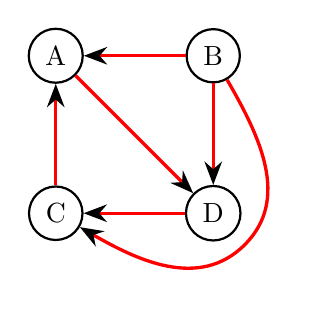
\begin{tikzpicture}
                \begin{scope}[every node/.style={circle,thick,draw}]
                    \node (A) at (0,2) {A};
                    \node (B) at (2,2) {B};
                    \node (C) at (0,0) {C};
                    \node (D) at (2,0) {D};
                \end{scope}
                \begin{scope}[>={Stealth[black]}, every edge/.style={draw=red,very thick}]
                    \path [->] (A) edge (D);
                    \path [->] (B) edge (A);
                    \path [->] (B) edge (D);
                    \path [->] (C) edge (A);
                    \path [->] (D) edge (C);
                    \draw [very thick,draw=red,->] (B) to[out=-60,in=45] (2.40,-0.40) to[out=-135,in=-30] (C);
                \end{scope}
            \end{tikzpicture}
        \end{column}
        \begin{column}{0.70\textwidth}
            \small
            \begin{align*}
                \mathbf{W}_0&=\kbordermatrix{
                               & \text{A} & \text{B} & \text{C} & \text{D} \\
                      \text{A} & \onslide<2-3>{\tikzmarkin[ver=style red]{col 1}}\onslide<4-7>{\tikzmarkin[hor=style red]{row 1}}0 & 0 & 0 & 1\onslide<4-7>{\tikzmarkend{row 1}} \\
                      \text{B} & \onslide<4-5>{\tikzmarkin[hor=style green]{row 2}}1 & 0 & 1 & 1\onslide<4-5>{\tikzmarkend{row 2}} \\
                      \text{C} & \onslide<6-7>{\tikzmarkin[hor=style green]{row 3}}1 & 0 & 0 & 0\onslide<6-7>{\tikzmarkend{row 3}} \\
                      \text{D} & 0\onslide<2-3>{\tikzmarkend{col 1}} & 0 & 1 & 0
                }
                &\mathbf{W}_1&=\kbordermatrix{
                               & \text{A} & \text{B} & \text{C} & \text{D} \\
                      \text{A} & \onslide<3->{0} & \onslide<9-10>{\tikzmarkin[ver=style red]{col 2}}\onslide<3->{0} & \onslide<3->{0} & \onslide<3->{1} \\
                      \text{B} & \onslide<4>{\tikzmarkin[hor=style green]{row 4}}\onslide<5->{1} & \onslide<5->{0} & \onslide<5->{1} & \onslide<5->{1}\onslide<4>{\tikzmarkend{row 4}} \\
                      \text{C} & \onslide<6>{\tikzmarkin[hor=style green]{row 5}}\onslide<7->{1} & \onslide<7->{0} & \onslide<7->{0} & \onslide<7->{1}\onslide<6>{\tikzmarkend{row 5}} \\
                      \text{D} & \onslide<3->{0} & \onslide<3->{0}\onslide<9-10>{\tikzmarkend{col 2}} & \onslide<3->{1} & \onslide<3->{0}
                }\\
                \mathbf{W}_2&=\kbordermatrix{
                               & \text{A} & \text{B} & \text{C} & \text{D} \\
                      \text{A} & \onslide<10->{0} & \onslide<10->{0} & \onslide<12-13>{\tikzmarkin[ver=style red]{col 3}}\onslide<10->{0} & \onslide<10->{1} \\
                      \text{B} & \onslide<14-15>{\tikzmarkin[hor=style green]{row 7}}\onslide<10->{1} & \onslide<10->{0} & \onslide<10->{1} & \onslide<10->{1}\onslide<14-15>{\tikzmarkend{row 7}} \\
                      \text{C} & \onslide<14-17>{\tikzmarkin[hor=style red]{row 6}}\onslide<10->{1} & \onslide<10->{0} & \onslide<10->{0} & \onslide<10->{1}\onslide<14-17>{\tikzmarkend{row 6}} \\
                      \text{D} & \onslide<16-17>{\tikzmarkin[hor=style green]{row 8}}\onslide<10->{0} & \onslide<10->{0} & \onslide<10->{1}\onslide<12-13>{\tikzmarkend{col 3}} & \onslide<10->{0}\onslide<16-17>{\tikzmarkend{row 8}}
                }
                &\mathbf{W}_3&=\kbordermatrix{
                               & \text{A} & \text{B} & \text{C} & \text{D} \\
                      \text{A} & \onslide<20-21>{\tikzmarkin[hor=style green]{row 12}}\onslide<13->{0} & \onslide<13->{0} & \onslide<13->{0} & \onslide<19>{\tikzmarkin[ver=style red]{col 4}}\onslide<13->{1}\onslide<20-21>{\tikzmarkend{row 12}} \\
                      \text{B} & \onslide<22-23>{\tikzmarkin[hor=style green]{row 13}}\onslide<14>{\tikzmarkin[hor=style green]{row 9}}\onslide<15->{1} & \onslide<15->{0} & \onslide<15->{1} & \onslide<15->{1}\onslide<14>{\tikzmarkend{row 9}}\onslide<22-23>{\tikzmarkend{row 13}} \\
                      \text{C} & \onslide<24-25>{\tikzmarkin[hor=style green]{row 14}}\onslide<13->{1} & \onslide<13->{0} & \onslide<13->{0} & \onslide<13->{1}\onslide<24-25>{\tikzmarkend{row 14}} \\
                      \text{D} & \onslide<26-27>{\tikzmarkin[hor=style orange]{row 19}}\onslide<20-25>{\tikzmarkin[hor=style red]{row 11}}\onslide<16>{\tikzmarkin[hor=style green]{row 10}}\onslide<17->{1} & \onslide<17->{0} & \onslide<17->{1} & \onslide<17->{1}\onslide<16>{\tikzmarkend{row 10}}\onslide<19>{\tikzmarkend{col 4}}\onslide<20-25>{\tikzmarkend{row 11}}\onslide<26-27>{\tikzmarkend{row 19}}
                }
            \end{align*}
            \[\mathbf{W}_4=\kbordermatrix{
                         & \text{A} & \text{B} & \text{C} & \text{D} \\
                \text{A} & \onslide<20>{\tikzmarkin[hor=style green]{row 15}}\onslide<21->{1 & 0 & 1 & 1}\onslide<20>{\tikzmarkend{row 15}} \\
                \text{B} & \onslide<22>{\tikzmarkin[hor=style green]{row 16}}\onslide<23->{1 & 0 & 1 & 1}\onslide<22>{\tikzmarkend{row 16}} \\
                \text{C} & \onslide<24>{\tikzmarkin[hor=style green]{row 17}}\onslide<25->{1 & 0 & 1 & 1}\onslide<24>{\tikzmarkend{row 17}} \\
                \text{D} & \onslide<26>{\tikzmarkin[hor=style green]{row 18}}\onslide<27-28>{1 & 0 & 1 & 1}\onslide<26>{\tikzmarkend{row 18}}
            }\]
        \end{column}
    \end{columns}
\end{frame}
\section{Kürzeste Wege}
\begin{frame}{Kürzeste Wege}
    yo
\end{frame}
\subsection{Dijkstra's Algorithmus}
\begin{frame}{Dijkstra's Algorithmus}
    jawohl
\end{frame}
\begin{frame}[t]{Beispiel: Dijkstra's Algorithmus}
    \begin{columns}
        \begin{column}{0.70\textwidth}
            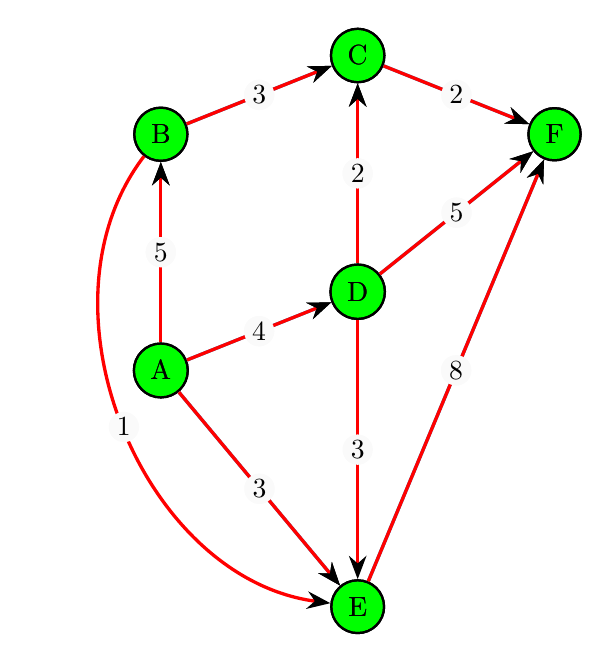
\begin{tikzpicture}
                \begin{scope}[every node/.style={circle,thick,draw}]
                    \alt<4->{\node[fill=green] (A) at (0,0) {A};}{\node (A) at (0,0) {A};}
                    \alt<15->{\node[fill=green] (B) at (0,3) {B};}{\node (B) at (0,3) {B};}
                    \alt<18->{\node[fill=green] (C) at (2.5,4) {C};}{\node (C) at (2.5,4) {C};}
                    \alt<10->{\node[fill=green] (D) at (2.5,1) {D};}{\node (D) at (2.5,1) {D};}
                    \alt<7->{\node[fill=green] (E) at (2.5,-3) {E};}{\node (E) at (2.5,-3) {E};}
                    \alt<21->{\node[fill=green] (F) at (5,3) {F};}{\node (F) at (5,3) {F};}
                \end{scope}

                \begin{scope}[>={Stealth[black]},every node/.style={inner sep=1pt,fill={rgb,255:red,250;green,250;blue,250},circle},every edge/.style={draw=red,very thick}]
                    \alt<5>{\path [->] (A) edge[draw=cyan] node {$5$} (B);}{\path [->] (A) edge node {$5$} (B);}
                    \alt<16>{\path [->] (B) edge[draw=cyan] node {$3$} (C);}{\path [->] (B) edge node {$3$} (C);}
                    \alt<5>{\path [->] (A) edge[draw=cyan] node {$4$} (D);}{\path [->] (A) edge node {$4$} (D);}
                    \alt<11>{\path [->] (D) edge[draw=cyan] node {$2$} (C);}{\path [->] (D) edge node {$2$} (C);}
                    \alt<5>{\path [->] (A) edge[draw=cyan] node {$3$} (E);}{\path [->] (A) edge node {$3$} (E);}
                    \path [->] (D) edge node {$3$} (E);
                    \alt<13>{\path [->] (D) edge[draw=cyan] node {$5$} (F);}{\path [->] (D) edge node {$5$} (F);}
                    \alt<19>{\path [->] (C) edge[draw=cyan] node {$2$} (F);}{\path [->] (C) edge node {$2$} (F);}
                    \alt<8>{\path [->] (E) edge[draw=cyan] node {$8$} (F);}{\path [->] (E) edge node {$8$} (F);}
                    \path [->] (B) edge[bend right=60] node {$1$} (E);
                \end{scope}
            \end{tikzpicture}
        \end{column}
        \begin{column}{0.30\textwidth}
            \begin{tabular}{c|c|c}
                $v$ & $d(v)$ & $p(v)$ \\
                \hline
                \onslide<4->{\tikzmarkin[hor=style green]{n1}}A & \onslide<2->{$0$} & \onslide<2->{$\varnothing$}\onslide<4->{\tikzmarkend{n1}} \\
                \onslide<15->{\tikzmarkin[hor=style green]{n10}}\onslide<6>{\tikzmarkin[hor=style red]{n2}}B & \onslide<3->{\alt<6->{$5$}{$\infty$}} & \onslide<3->{\alt<6->{A}{$\varnothing$}}\onslide<6>{\tikzmarkend{n2}}\onslide<15->{\tikzmarkend{n10}} \\
                \onslide<18->{\tikzmarkin[hor=style green]{n11}}\onslide<12>{\tikzmarkin[hor=style red]{n8}}C & \onslide<3->{\alt<12->{$6$}{$\infty$}} & \onslide<3->{\alt<12->{D}{$\varnothing$}}\onslide<12>{\tikzmarkend{n8}}\onslide<18->{\tikzmarkend{n11}} \\
                \onslide<10->{\tikzmarkin[hor=style green]{n7}}\onslide<6>{\tikzmarkin[hor=style red]{n3}}D & \onslide<3->{\alt<6->{$4$}{$\infty$}} & \onslide<3->{\alt<6->{A}{$\varnothing$}}\onslide<6>{\tikzmarkend{n3}}\onslide<10->{\tikzmarkend{n7}} \\
                \onslide<7->{\tikzmarkin[hor=style green]{n5}}\onslide<6>{\tikzmarkin[hor=style red]{n4}}E & \onslide<3->{\alt<6->{$3$}{$\infty$}} & \onslide<3->{\alt<6->{A}{$\varnothing$}}\onslide<6>{\tikzmarkend{n4}}\onslide<7->{\tikzmarkend{n5}} \\
                \onslide<21->{\tikzmarkin[hor=style green]{n13}}\onslide<20>{\tikzmarkin[hor=style red]{n12}}\onslide<14>{\tikzmarkin[hor=style red]{n9}}\onslide<9>{\tikzmarkin[hor=style red]{n6}}F & \onslide<3->{\alt<20->{$8$}{\alt<14->{$9$}{\alt<9->{$11$}{$\infty$}}}} & \onslide<3->{\alt<20->{C}{\alt<14->{D}{\alt<9->{E}{$\varnothing$}}}}\onslide<9>{\tikzmarkend{n6}}\onslide<14>{\tikzmarkend{n9}}\onslide<20>{\tikzmarkend{n12}}\onslide<21->{\tikzmarkend{n13}}
            \end{tabular}
        \end{column}
    \end{columns}
\end{frame}
\begin{frame}{Blocks}
\begin{block}{Block Title}
You can also highlight sections of your presentation in a block, with it's own title
\end{block}
\begin{theorem}
There are separate environments for theorems, examples, definitions, lemmas and proofs.
\end{theorem}
\begin{lemma}
    \[\sum_{v\in V}\deg^-(v)=\sum_{v\in V}\deg^+(v)=|E|\]
\end{lemma}
\begin{proof}
    Left as an exercise to the reader.
\end{proof}
\begin{example}
Here is an example of an example block.
\end{example}
\end{frame}

% Placing a * after \section means it will not show in the
% outline or table of contents.
\section*{Summary}

\begin{frame}{Summary}
    \begin{itemize}
    \item
        The \alert{first main message} of your talk in one or two lines.
    \item
        The \alert{second main message} of your talk in one or two lines.
    \item
        Perhaps a \alert{third message}, but not more than that.
    \end{itemize}

    \begin{itemize}
    \item
        Outlook
        \begin{itemize}
        \item
            Something you haven't solved.
        \item
            Something else you haven't solved.
        \end{itemize}
    \end{itemize}
\end{frame}



% All of the following is optional and typically not needed.
\appendix
\section<presentation>*{\appendixname}
\subsection<presentation>*{For Further Reading}

\begin{frame}[allowframebreaks]
    \frametitle<presentation>{For Further Reading}

    \begin{thebibliography}{10}

    \beamertemplatebookbibitems
    % Start with overview books.

    \bibitem{Author1990}
        A.~Author.
        \newblock {\em Handbook of Everything}.
        \newblock Some Press, 1990.


    \beamertemplatearticlebibitems
    % Followed by interesting articles. Keep the list short.

    \bibitem{Someone2000}
        S.~Someone.
        \newblock On this and that.
        \newblock {\em Journal of This and That}, 2(1):50--100,
        2000.
    \end{thebibliography}
\end{frame}

\end{document}